%!TEX root = ../main.tex
\chapter{Design}

After planning out the requirements, the next step in the design of KidQuest was to plan out the database structure.
I created an entity relationship to map out the various tables needed and the relationships between them.

\begin{figure}[t]
	\centering
	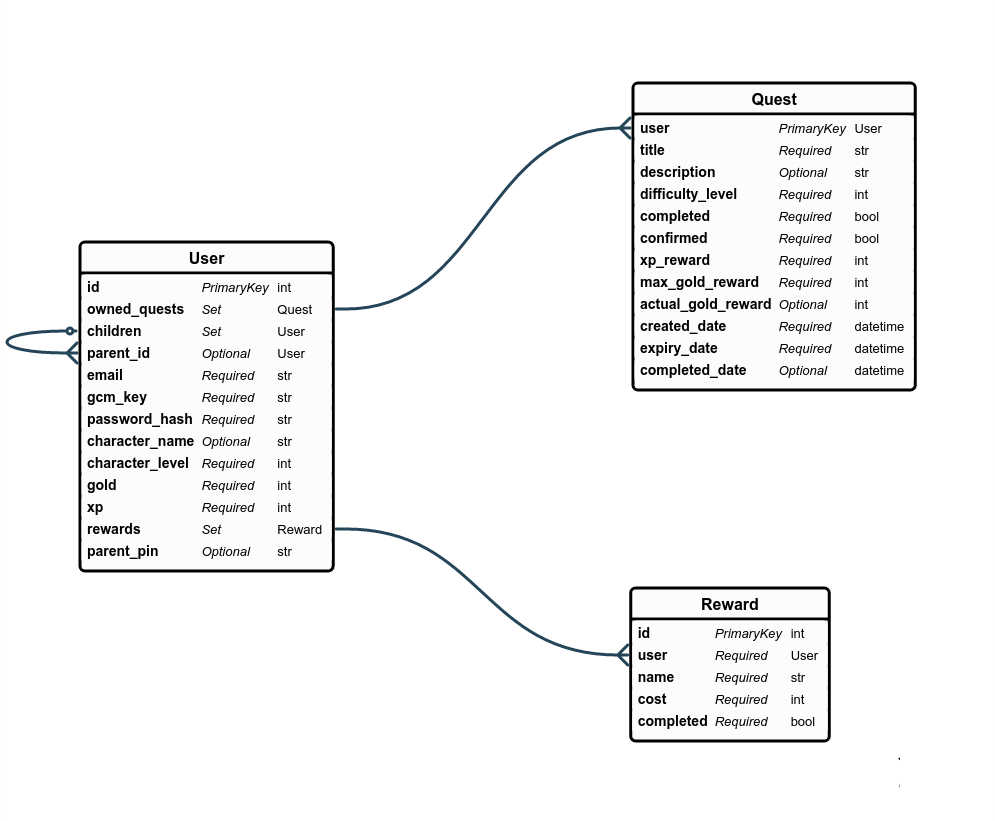
\includegraphics[width=0.75\textwidth]{images/entityRelationshipDiagram.png}
	\caption{Entity-Relationship Diagram}
	\label{fig:ERD}
\end{figure}

I have chosen to create the application in the Android SDK largely due to my previous experience with Java and Android. 
Furthermore, I believe Android is more applicable to the target audience of the app, as Android owns 82.8\% of the smartphone market share as of 2015.
%http://www.idc.com/prodserv/smartphone-os-market-share.jsp
I believe that parents are also more likely to buy their children Android phones than other brands due to the lower price point, making them more appealing when considering the likelihood of them being lost or broken by a child.

For the data analytics, I have opted to use web services written in Flask microframework for python, hosted on a server running Ubuntu Server 14.04. 
I have chosen python due to it's strong backing and community support in data analytics, and is one of the main languages of choice for scientists and statisticians.
The flask framework was chosen specifically as it is very simple to write and host RESTful APIs over the web.

To safely store and version control the code, I used a GitHub private repository to host my code in cloud storage and allow for me to better manage changes to the code-base. 

\section{Aesthetic Design}

\subsection{Wireframes}

\subsection{Android Developer Guidelines}

\section{Usability}

\section{Use Cases}	

\section{Development Style}
